\section{Unterteilungen und Minoren}

\textbf{Definition}: Sei $G=(V,E)$ ein Graph, $e=uv$ eine Kante. Dann ist die \textbf{Unterteilung von $\boldsymbol{e}$ in $\boldsymbol{G}$} der Graph $G\circ e=(V',E')$ mit
\begin{itemize}
	\item $V'=V+\{w\}$
	\item $E'=(E\setminus \{uv\})+\{uw,vw\}$
\end{itemize}
\bigskip
\textbf{Beobachtung}: $G$ planar $\iff$ $G\circ e$ planar\\

\textbf{Definition}: Graph $G$ ist eine \textbf{Unterteilung von $\boldsymbol{H}$} wenn $G=((H \circ e_1)\circ e_2)\cdots)\circ e_k$.
Wir sagen auch $G$ ist $\boldsymbol{H}$\textbf{-Unterteilung}.
Graph $G$ \textbf{enthält eine $\boldsymbol{H}$-Unterteilung}, wenn ein Teilgraph $G'\subseteq G$ eine $H$-Unterteilung ist.

\begin{center}
	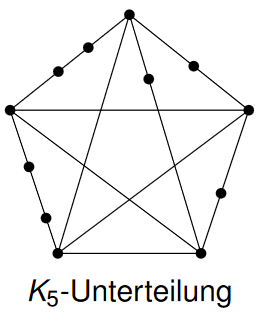
\includegraphics[width=0.17\textwidth]{images/k5-unterteilung.png}
\end{center}

\textbf{Beobachtung}: 
\begin{itemize}
	\item $K_5$- und $K_{3,3}$-Unterteilungen sind nicht-planar
	\item Jeder Graph der eine $K_5$ oder $K_{3,3}$-Unterteilung enthält, ist nicht planar
\end{itemize}
\bigskip
\textbf{Satz von Kuratowski}: $G$ ist planar $\iff$ $G$ enthält keine $K_5$- oder $K_{3,3}$-Unterteilung